
\documentclass[10pt, aspectratio=169, xcolor={dvipsnames,svgnames,table}]{beamer}

\usetheme[progressbar=frametitle]{metropolis}
\usepackage{appendixnumberbeamer}
\usepackage[flushleft]{threeparttable}

\usepackage{booktabs}
\usepackage[scale=2]{ccicons}
\usepackage{eurosym}
\usepackage{ragged2e}
\usepackage{setspace}
\usepackage{dsfont}
\usepackage{subcaption}
\usepackage{tikz}

\newenvironment{fignotes}{\tiny}

\newenvironment{fignotes2}{\begin{quote}\scriptsize}{\end{quote}}

% Color
\definecolor{ebrd_blue}{HTML}{0E5599}

\definecolor{gray}{gray}{0.9}

% Redefine beamergotobutton style
\setbeamercolor{button}{bg=gray,fg=ebrd_blue}

\hypersetup{
     colorlinks   = true,
     citecolor    = ebrd_blue,
     linkcolor    = ebrd_blue,
     urlcolor    = ebrd_blue
}

\usepackage{pgfplots}
\usepgfplotslibrary{dateplot}

\usepackage{xspace}
\newcommand{\themename}{\textbf{\textsc{metropolis}}\xspace}
\def\sym#1{\ifmmode^{#1}\else\(^{#1}\)\fi}

\definecolor{MyBackground}{RGB}{255,255,255}
\setbeamercolor{background canvas}{bg=MyBackground} % set background color to white

\title[Some age-cohort regressions]{Age-cohort regressions with ESS-MPD matched data}
%\subtitle{Chapter 4 TR 2025-26}
\author[ESS-MPD project]{ESS-MPD project}

\date{\normalsize \vspace{0.2cm} April 2026}

\makeatletter
\setbeamertemplate{title page}{
  \begin{minipage}[b][\paperheight]{\textwidth}
    \centering
    \ifx\inserttitlegraphic\@empty\else\usebeamertemplate*{title graphic}\fi
    \vfill%
    \ifx\inserttitle\@empty\else\usebeamertemplate*{title}\fi
    \ifx\insertsubtitle\@empty\else\usebeamertemplate*{subtitle}\fi
    \usebeamertemplate*{title separator}
    \ifx\beamer@shortauthor\@empty\else\usebeamertemplate*{author}\fi
    \ifx\insertdate\@empty\else\usebeamertemplate*{date}\fi
    \ifx\insertinstitute\@empty\else\usebeamertemplate*{institute}\fi
    \vfill
    \vspace*{1mm}
  \end{minipage}
}

\setbeamertemplate{title}{
  \linespread{1.0}%
  \inserttitle%
  \par%
  \vspace*{0.5em}
}
\setbeamertemplate{subtitle}{
  \insertsubtitle%
  \par%
  \vspace*{0.5em}
}
\makeatother


\usepackage{background}

\newcommand{\switchbackground}[3][0.05]{%
}

\setbeamertemplate{frame footer}{\hspace{0.7em} \insertshortauthor\hfill\insertshorttitle\hfill April 2026 \hspace{0.7em} \insertframenumber/\inserttotalframenumber \hspace{0.7em} \smallskip}
\setbeamerfont{page number in head/foot}{size=\tiny}

\setbeamertemplate{footline}{%
    \begin{beamercolorbox}[wd=\textwidth, sep=1ex]{footline}
        \usebeamerfont{page number in head/foot}%
        \usebeamertemplate*{frame footer}
        \hfill%
    \end{beamercolorbox}%
}

\setbeamerfont{page number in head/foot}{size=\tiny}

% Color
\definecolor{ebrd_blue}{HTML}{00529B}

\hypersetup{
     colorlinks   = true,
     citecolor    = ebrd_blue,
     linkcolor    = ebrd_blue
}

\setbeamercolor{progress bar}{fg=ebrd_blue}
\setbeamercolor{alerted text}{fg=ebrd_blue}
\setbeamercolor{frametitle}{bg=ebrd_blue}

\usepackage[english]{babel}
\usepackage{natbib}
\bibliographystyle{authordate3}
\setcitestyle{authoryear,open={(},close={)}}

\usepackage[default,scaled=0.8]{librefranklin}
\usepackage[T1]{fontenc}
\linespread{1}

\setbeamertemplate{itemize item}{\scriptsize$\bullet$}
\setbeamertemplate{itemize subitem}{\scriptsize$\blacktriangleright$}
\setbeamertemplate{itemize subsubitem}{\scriptsize$\diamond$}

% Section title pages
\metroset{sectionpage=progressbar}

\begin{document}

\maketitle

% \section{Note on MPD coverage}
%
% \begin{frame} % ---------------------------------------------------------
% \frametitle{Note on MPD per-code coverage}
%
% The MPD coding scheme has three layers of categories:
% \begin{enumerate}
%     \item \textbf{Main categories} (3-digit, per101--per706): available in \textit{all} handbook versions for \textit{all} countries
%     \item \textbf{CEE sub-codes} (4-digit, per1011--per7062): introduced in handbook~v1 (2001) for \textbf{Central \& Eastern European transitional democracies}. These were gradually abandoned as issues were absorbed into the main categories
%     \item \textbf{V5 subcategories} (decimal, per103\_1--per703\_2): introduced in handbook~v5 (2021) for all countries
% \end{enumerate}
%
% \vspace{0.1cm}
% Eight per-codes in our original index definitions are CEE sub-codes. They were only ever coded for a subset of CEE elections (\textbf{10--70\%} of party-elections in 2000--2014) and have \textbf{0\% availability from 2015 onwards}. I therefore \textbf{drop} them from the index computation in this analysis. The remaining per-codes are all main categories with \textbf{$\sim$100\%} coverage across all ESS waves.
%
% \vspace{0.1cm}
% \hyperlink{appendix:econ}{\beamerskipbutton{Economic components}} \hyperlink{appendix:cult}{\beamerskipbutton{Cultural components}} \hyperlink{appendix:coverage_econ}{\beamerskipbutton{Economic heatmap}} \hyperlink{appendix:coverage_cult}{\beamerskipbutton{Cultural heatmap}}
%
% \end{frame} % ---------------------------------------------------------


\section{Regressions}

\begin{frame} % ---------------------------------------------------------
\frametitle{Raw composite indices (TR sample + top-up)}
\centering
\vspace{-0.5cm}
{\footnotesize
\begin{equation*}
    \underbrace{MPD_{it}}_{\substack{\text{Composite} \\ \text{index}}} = \alpha \; + \underbrace{\sum_{k} \beta_k \mathbf{1}\{Age_{it} \in \text{Cat}_k\}}_{\substack{\text{Age category dummies} \\ \text{(omitting 18-34)}}} \; + \underbrace{\mathbf{X_{it}'}\Theta}_{\substack{\text{Vector of} \\ \text{controls}}} + \underbrace{\gamma_{ct}}_{\substack{\text{Country $\times$ election} \\ \text{year FEs}}} + \underbrace{\eta_{g}}_{\substack{\text{Generation} \\ \text{FEs}}} + \varepsilon_{it}
\end{equation*}
}
\vspace{-1.2cm}
    \begin{table}[H]
    \centering
    \resizebox{0.52\textwidth}{!}{%
        \begin{threeparttable}[H]
        \centering
        \captionsetup{justification=centering}
        \caption*{}\label{tab:raw_TR}
        {
\def\sym#1{\ifmmode^{#1}\else\(^{#1}\)\fi}
\begin{tabular}{l*{6}{c}}
\toprule
                    &\multicolumn{3}{c}{Economic index}                               &\multicolumn{3}{c}{Cultural index}                               \\\cmidrule(lr){2-4}\cmidrule(lr){5-7}
                    &\multicolumn{1}{c}{(1)}         &\multicolumn{1}{c}{(2)}         &\multicolumn{1}{c}{(3)}         &\multicolumn{1}{c}{(4)}         &\multicolumn{1}{c}{(5)}         &\multicolumn{1}{c}{(6)}         \\
\midrule
35-49               &      -0.012         &       0.001         &       0.005         &       0.026\sym{**} &       0.014         &       0.028         \\
                    &     (0.013)         &     (0.013)         &     (0.007)         &     (0.010)         &     (0.012)         &     (0.019)         \\
50-64               &      -0.010         &      -0.007         &      -0.009         &       0.033\sym{*}  &       0.008         &       0.036         \\
                    &     (0.030)         &     (0.029)         &     (0.012)         &     (0.017)         &     (0.020)         &     (0.027)         \\
65+                 &      -0.068         &      -0.089\sym{**} &      -0.061\sym{*}  &       0.063\sym{*}  &       0.025         &       0.043         \\
                    &     (0.042)         &     (0.043)         &     (0.031)         &     (0.031)         &     (0.038)         &     (0.039)         \\
Baby Boomers (1946-1964)&                     &                     &       0.053\sym{**} &                     &                     &      -0.022         \\
                    &                     &                     &     (0.025)         &                     &                     &     (0.014)         \\
Generation X (1965-1980)&                     &                     &       0.024\sym{*}  &                     &                     &       0.011         \\
                    &                     &                     &     (0.013)         &                     &                     &     (0.017)         \\
Millennials and Gen Z (post-1981)&                     &                     &       0.050\sym{**} &                     &                     &       0.013         \\
                    &                     &                     &     (0.021)         &                     &                     &     (0.027)         \\
\midrule
R-squared           &       0.351         &       0.356         &       0.356         &       0.263         &       0.272         &       0.272         \\
Observations        &      256947         &      255219         &      255219         &      256947         &      255219         &      255219         \\
Country $\times$ election year FEs&    $\times$         &    $\times$         &    $\times$         &    $\times$         &    $\times$         &    $\times$         \\
Generational cohort FEs&                     &                     &    $\times$         &                     &                     &    $\times$         \\
Controls            &                     &    $\times$         &    $\times$         &                     &    $\times$         &    $\times$         \\
Mean of outcome     &       1.803         &       1.803         &       1.803         &      -0.056         &      -0.056         &      -0.056         \\
SD of outcome       &       0.961         &       0.960         &       0.960         &       0.863         &       0.863         &       0.863         \\
\bottomrule
\end{tabular}
}

        \begin{tablenotes}[para,flushleft]
        \scriptsize
        \textbf{Notes}: TR sample + top-up. Standard errors clustered at the country level in parentheses. Economic index: higher $=$ more left-wing. Cultural index: higher $=$ more traditional/sovereignty. Significance levels: * $p<.1$, ** $p<.05$, *** $p<.01$.
        \end{tablenotes}
        \end{threeparttable}
    }
    \end{table}
\end{frame} % ---------------------------------------------------------


\begin{frame} % ---------------------------------------------------------
\frametitle{Standardized composite indices, z-scored (TR sample + top-up)}
\centering
\vspace{-0.5cm}
{\footnotesize
\begin{equation*}
    \underbrace{MPD_{it}^{z}}_{\substack{\text{z-scored} \\ \text{index}}} = \alpha \; + \underbrace{\sum_{k} \beta_k \mathbf{1}\{Age_{it} \in \text{Cat}_k\}}_{\substack{\text{Age category dummies} \\ \text{(omitting 18-34)}}} \; + \underbrace{\mathbf{X_{it}'}\Theta}_{\substack{\text{Vector of} \\ \text{controls}}} + \underbrace{\gamma_{ct}}_{\substack{\text{Country $\times$ election} \\ \text{year FEs}}} + \underbrace{\eta_{g}}_{\substack{\text{Generation} \\ \text{FEs}}} + \varepsilon_{it}
\end{equation*}
}
\vspace{-1.2cm}
    \begin{table}[H]
    \centering
    \resizebox{0.52\textwidth}{!}{%
        \begin{threeparttable}[H]
        \centering
        \captionsetup{justification=centering}
        \caption*{}\label{tab:std_TR}
        {
\def\sym#1{\ifmmode^{#1}\else\(^{#1}\)\fi}
\begin{tabular}{l*{6}{c}}
\toprule
                    &\multicolumn{3}{c}{Economic index}                               &\multicolumn{3}{c}{Cultural index}                               \\\cmidrule(lr){2-4}\cmidrule(lr){5-7}
                    &\multicolumn{1}{c}{(1)}         &\multicolumn{1}{c}{(2)}         &\multicolumn{1}{c}{(3)}         &\multicolumn{1}{c}{(4)}         &\multicolumn{1}{c}{(5)}         &\multicolumn{1}{c}{(6)}         \\
\midrule
35-49               &      -0.014         &       0.001         &       0.005         &       0.032\sym{**} &       0.017         &       0.034         \\
                    &     (0.015)         &     (0.015)         &     (0.008)         &     (0.012)         &     (0.014)         &     (0.023)         \\
50-64               &      -0.012         &      -0.008         &      -0.011         &       0.040\sym{*}  &       0.009         &       0.043         \\
                    &     (0.035)         &     (0.034)         &     (0.014)         &     (0.020)         &     (0.024)         &     (0.032)         \\
65+                 &      -0.078         &      -0.102\sym{**} &      -0.070\sym{*}  &       0.076\sym{*}  &       0.030         &       0.051         \\
                    &     (0.048)         &     (0.050)         &     (0.035)         &     (0.038)         &     (0.045)         &     (0.047)         \\
Baby Boomers (1946-1964)&                     &                     &       0.061\sym{**} &                     &                     &      -0.026         \\
                    &                     &                     &     (0.029)         &                     &                     &     (0.017)         \\
Generation X (1965-1980)&                     &                     &       0.028\sym{*}  &                     &                     &       0.013         \\
                    &                     &                     &     (0.015)         &                     &                     &     (0.020)         \\
Millennials and Gen Z (post-1981)&                     &                     &       0.057\sym{**} &                     &                     &       0.016         \\
                    &                     &                     &     (0.024)         &                     &                     &     (0.032)         \\
\midrule
R-squared           &       0.351         &       0.356         &       0.356         &       0.263         &       0.272         &       0.272         \\
Observations        &      256947         &      255219         &      255219         &      256947         &      255219         &      255219         \\
Country $\times$ election year FEs&    $\times$         &    $\times$         &    $\times$         &    $\times$         &    $\times$         &    $\times$         \\
Generational cohort FEs&                     &                     &    $\times$         &                     &                     &    $\times$         \\
Controls            &                     &    $\times$         &    $\times$         &                     &    $\times$         &    $\times$         \\
Mean of outcome     &       0.044         &       0.044         &       0.044         &      -0.033         &      -0.033         &      -0.033         \\
SD of outcome       &       1.102         &       1.101         &       1.101         &       1.037         &       1.037         &       1.037         \\
\bottomrule
\end{tabular}
}

        \begin{tablenotes}[para,flushleft]
        \scriptsize
        \textbf{Notes}: TR sample + top-up. Standard errors clustered at the country level in parentheses. Both indices z-scored across all observations. Significance levels: * $p<.1$, ** $p<.05$, *** $p<.01$.
        \end{tablenotes}
        \end{threeparttable}
    }
    \end{table}
\end{frame} % ---------------------------------------------------------


\begin{frame} % ---------------------------------------------------------
\frametitle{PCA composite indices, PC1 (TR sample + top-up)}
\centering
\vspace{-0.5cm}
{\footnotesize
\begin{equation*}
    \underbrace{MPD_{it}^{PC1}}_{\substack{\text{PCA} \\ \text{index}}} = \alpha \; + \underbrace{\sum_{k} \beta_k \mathbf{1}\{Age_{it} \in \text{Cat}_k\}}_{\substack{\text{Age category dummies} \\ \text{(omitting 18-34)}}} \; + \underbrace{\mathbf{X_{it}'}\Theta}_{\substack{\text{Vector of} \\ \text{controls}}} + \underbrace{\gamma_{ct}}_{\substack{\text{Country $\times$ election} \\ \text{year FEs}}} + \underbrace{\eta_{g}}_{\substack{\text{Generation} \\ \text{FEs}}} + \varepsilon_{it}
\end{equation*}
}
\vspace{-1.2cm}
    \begin{table}[H]
    \centering
    \resizebox{0.52\textwidth}{!}{%
        \begin{threeparttable}[H]
        \centering
        \captionsetup{justification=centering}
        \caption*{}\label{tab:pca_TR}
        {
\def\sym#1{\ifmmode^{#1}\else\(^{#1}\)\fi}
\begin{tabular}{l*{6}{c}}
\toprule
                    &\multicolumn{3}{c}{Economic index}                               &\multicolumn{3}{c}{Cultural index}                               \\\cmidrule(lr){2-4}\cmidrule(lr){5-7}
                    &\multicolumn{1}{c}{(1)}         &\multicolumn{1}{c}{(2)}         &\multicolumn{1}{c}{(3)}         &\multicolumn{1}{c}{(4)}         &\multicolumn{1}{c}{(5)}         &\multicolumn{1}{c}{(6)}         \\
\midrule
35-49               &      -0.027         &      -0.007         &       0.005         &       0.035\sym{**} &       0.017         &       0.047         \\
                    &     (0.029)         &     (0.029)         &     (0.014)         &     (0.016)         &     (0.019)         &     (0.029)         \\
50-64               &      -0.020         &      -0.020         &      -0.021         &       0.041         &      -0.000         &       0.057         \\
                    &     (0.063)         &     (0.058)         &     (0.024)         &     (0.028)         &     (0.035)         &     (0.040)         \\
65+                 &      -0.128         &      -0.173\sym{*}  &      -0.126\sym{**} &       0.074         &       0.011         &       0.057         \\
                    &     (0.090)         &     (0.087)         &     (0.057)         &     (0.052)         &     (0.064)         &     (0.063)         \\
Baby Boomers (1946-1964)&                     &                     &       0.086\sym{**} &                     &                     &      -0.028         \\
                    &                     &                     &     (0.041)         &                     &                     &     (0.022)         \\
Generation X (1965-1980)&                     &                     &       0.028         &                     &                     &       0.028         \\
                    &                     &                     &     (0.022)         &                     &                     &     (0.031)         \\
Millennials and Gen Z (post-1981)&                     &                     &       0.089\sym{**} &                     &                     &       0.045         \\
                    &                     &                     &     (0.043)         &                     &                     &     (0.042)         \\
\midrule
R-squared           &       0.272         &       0.276         &       0.277         &       0.228         &       0.237         &       0.237         \\
Observations        &      256947         &      255219         &      255219         &      256947         &      255219         &      255219         \\
Country $\times$ election year FEs&    $\times$         &    $\times$         &    $\times$         &    $\times$         &    $\times$         &    $\times$         \\
Generational cohort FEs&                     &                     &    $\times$         &                     &                     &    $\times$         \\
Controls            &                     &    $\times$         &    $\times$         &                     &    $\times$         &    $\times$         \\
Mean of outcome     &      -0.012         &      -0.012         &      -0.012         &      -0.054         &      -0.053         &      -0.053         \\
SD of outcome       &       1.534         &       1.534         &       1.534         &       1.377         &       1.378         &       1.378         \\
\bottomrule
\end{tabular}
}

        \begin{tablenotes}[para,flushleft]
        \scriptsize
        \textbf{Notes}: TR sample + top-up. Standard errors clustered at the country level in parentheses. PC1 within each bundle, sign-aligned with raw index. Significance levels: * $p<.1$, ** $p<.05$, *** $p<.01$.
        \end{tablenotes}
        \end{threeparttable}
    }
    \end{table}
\end{frame} % ---------------------------------------------------------


\section{Polarization}

\begin{frame} % ---------------------------------------------------------
\frametitle{Polarization over time: economic vs.\ cultural dimension}

\begin{figure}[H]
    \begin{center}
    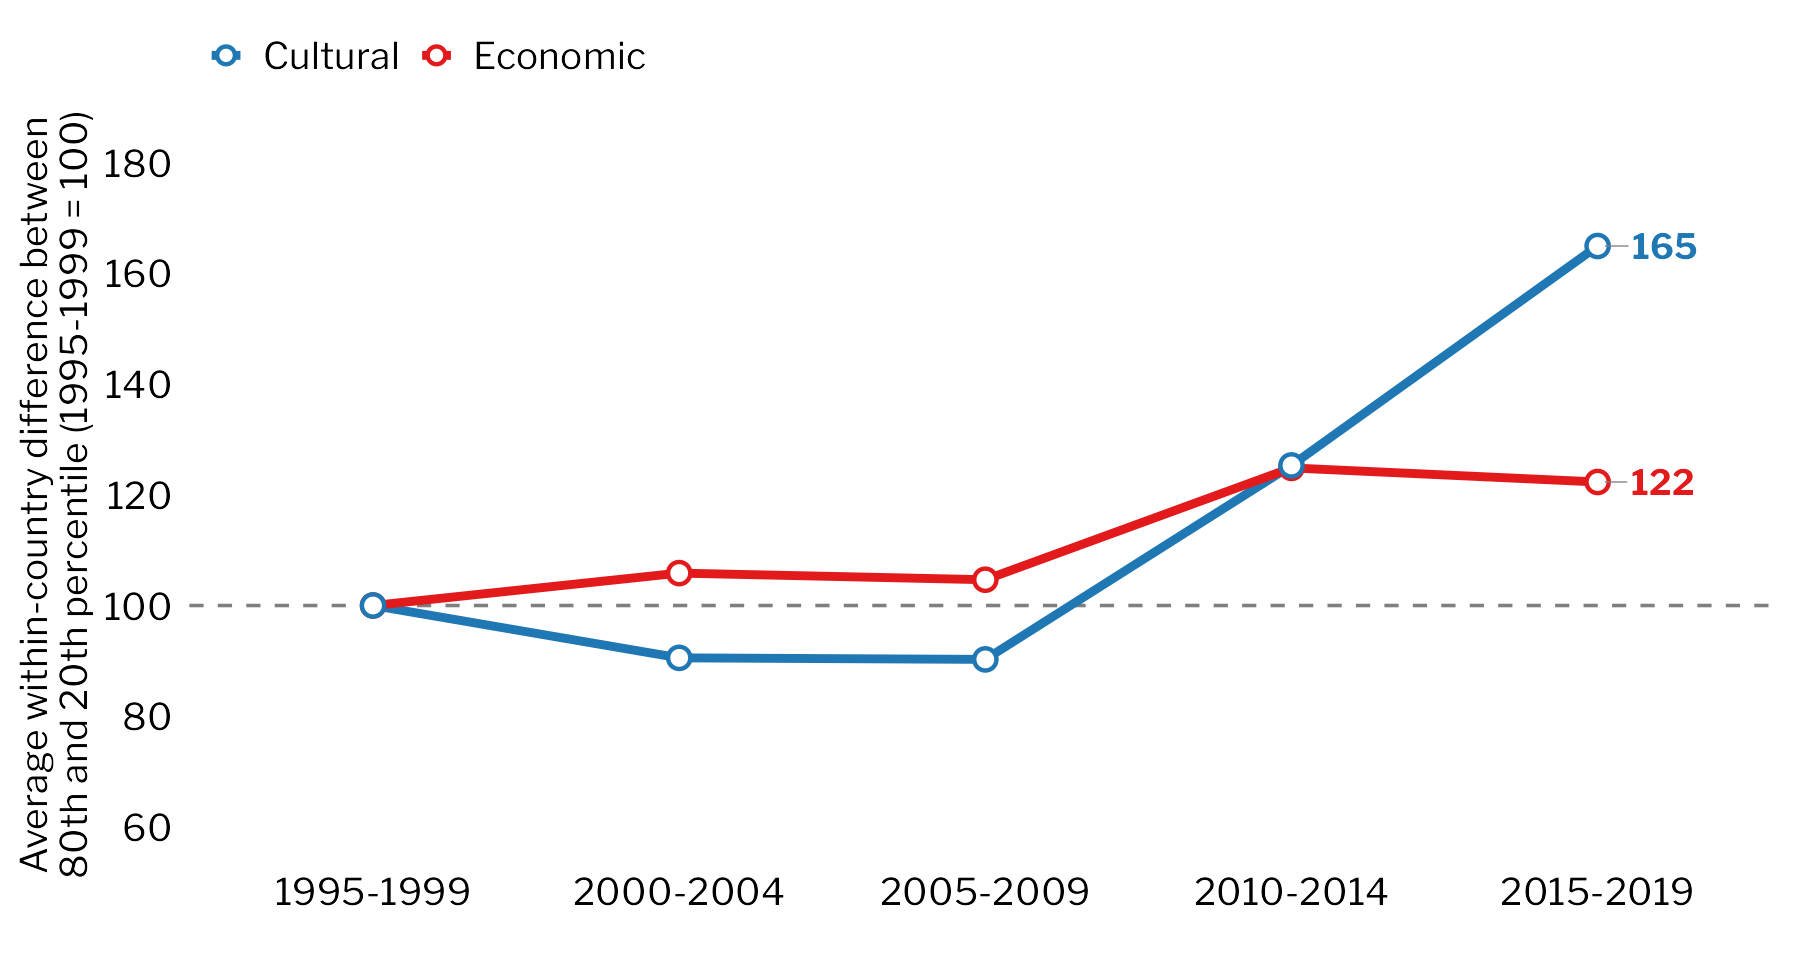
\includegraphics[width=0.85\textwidth]{../output/figures/mpd_charts_overttime/mpd_p82_combined.png}
    \end{center}
\end{figure}

\end{frame} % ---------------------------------------------------------


% \section{Appendix}
%
% \setcounter{table}{0}
% \setcounter{figure}{0}
% \renewcommand{\thesection}{A}
% \renewcommand{\thetable}{A\arabic{table}}
% \renewcommand{\thefigure}{A\arabic{figure}}
%
% \appendix
%
% \begin{frame} % ---------------------------------------------------------
% \frametitle{Appendix: Economic index components}\label{appendix:econ}
%
% \alert{\textbf{Economic index (raw)}}: higher $=$ more left-wing economics (pro-welfare / pro-regulation).
%
% \vspace{0.2cm}
% \begin{table}[H]
% \centering
% \resizebox{0.62\textwidth}{!}{%
% \begin{tabular}{@{} c l l @{}}
% \toprule
% \textbf{Sign} & \textbf{MPD code} & \textbf{Component} \\
% \midrule
% \multicolumn{3}{@{}l}{\textit{Market vs.\ state / ownership / macro stance}} \\
% $-$ & per401  & Free market economy (laissez-faire, private enterprise) \\
% $+$ & per403  & Market regulation / social market economy (competition policy, consumer protection) \\
% $+$ & per405  & Corporatism / tripartite coordination (state--employers--unions) \\
% $+$ & per412  & Direct government control of the economy (e.g.\ price controls, minimum wages) \\
% $+$ & per413  & Nationalisation / government ownership of industries or land \\
% $-$ & per414  & Economic orthodoxy (budget discipline, strong currency, traditional institutions) \\
% $+$ & per415  & Marxist--Leninist ideology / terminology (where applicable) \\
% \rowcolor{red!10} \textcolor{red}{$-$} & \textcolor{red}{per4012} & \textcolor{red}{Oppose direct government control \hfill\textit{[dropped --- CEE sub-code]}} \\
% \rowcolor{red!10} \textcolor{red}{$+$} & \textcolor{red}{per4123} & \textcolor{red}{Publicly-owned industries \hfill\textit{[dropped --- CEE sub-code]}} \\
% \rowcolor{red!10} \textcolor{red}{$+$} & \textcolor{red}{per4124} & \textcolor{red}{Socialist/cooperative property; anti-privatisation \hfill\textit{[dropped --- CEE sub-code]}} \\
% \midrule
% \multicolumn{3}{@{}l}{\textit{Redistribution / welfare / education / labour}} \\
% $+$ & per503  & Social justice / equality; protect underprivileged groups; anti-discrimination \\
% $+$ & per504  & Welfare state expansion (health, childcare, pensions, social housing) \\
% $-$ & per505  & Welfare state limitation (cutbacks; private care before state care) \\
% $+$ & per506  & Education expansion (improve/expand provision) \\
% $-$ & per507  & Education limitation (fees; private schools; limit public spending) \\
% $+$ & per701  & Pro-labour / unions; better jobs/wages/conditions; worker protection \\
% $-$ & per702  & Anti-labour / anti-union (e.g.\ unions abusing power) \\
% \rowcolor{red!10} \textcolor{red}{$-$} & \textcolor{red}{per5041} & \textcolor{red}{Private welfare provision \hfill\textit{[dropped --- CEE sub-code]}} \\
% \rowcolor{red!10} \textcolor{red}{$-$} & \textcolor{red}{per5061} & \textcolor{red}{Private education \hfill\textit{[dropped --- CEE sub-code]}} \\
% \bottomrule
% \end{tabular}
% }
% \end{table}
%
% \end{frame} % ---------------------------------------------------------
%
%
% \begin{frame} % ---------------------------------------------------------
% \frametitle{Appendix: Cultural index components}\label{appendix:cult}
%
% \alert{\textbf{Cultural index (raw)}}: higher $=$ more traditional values / anti-globalisation / sovereignty.
%
% \vspace{0.2cm}
% \begin{table}[H]
% \centering
% \resizebox{0.7\textwidth}{!}{%
% \begin{tabular}{@{} c l l @{}}
% \toprule
% \textbf{Sign} & \textbf{MPD code} & \textbf{Component} \\
% \midrule
% \multicolumn{3}{@{}l}{\textit{Globalisation / internationalism / EU scepticism}} \\
% $-$ & per107  & International cooperation (UN, international institutions, global governance) \\
% $-$ & per108  & Pro-EU / pro-European integration \\
% $+$ & per109  & Sovereignty / anti-internationalism; unilateralism \\
% $+$ & per110  & Anti-EU / EU scepticism (oppose EU authority/policies/budget contribution) \\
% \midrule
% \multicolumn{3}{@{}l}{\textit{National identity / traditional morality / diversity}} \\
% $+$ & per601  & Nationalism / patriotism; pride of citizenship; defend national way of life \\
% $-$ & per602  & Anti-nationalism / opposition to national pride and national ideas \\
% \rowcolor{red!10} \textcolor{red}{$+$} & \textcolor{red}{per2022} & \textcolor{red}{Restrictive citizenship / enfranchisement \hfill\textit{[dropped --- CEE sub-code]}} \\
% \rowcolor{red!10} \textcolor{red}{$-$} & \textcolor{red}{per2023} & \textcolor{red}{Lax citizenship / enfranchisement \hfill\textit{[dropped --- CEE sub-code]}} \\
% $+$ & per603  & Traditional / religious moral values; traditional family; role of religion \\
% $-$ & per604  & Social liberalism / opposition to traditional morality (divorce/abortion; church--state separation) \\
% $-$ & per607  & Multiculturalism / cultural diversity (pluralism, minority autonomy) \\
% $+$ & per608  & Assimilation / cultural homogeneity (anti-multiculturalism) \\
% \rowcolor{red!10} \textcolor{red}{$-$} & \textcolor{red}{per7062} & \textcolor{red}{Assistance to refugees / war-displaced persons \hfill\textit{[dropped --- CEE sub-code]}} \\
% \bottomrule
% \end{tabular}
% }
% \end{table}
%
% \end{frame} % ---------------------------------------------------------
%
%
% \begin{frame} % ---------------------------------------------------------
% \frametitle{Appendix: Economic index per-code availability}\label{appendix:coverage_econ}
%
% \begin{figure}[H]
%     \begin{center}
%     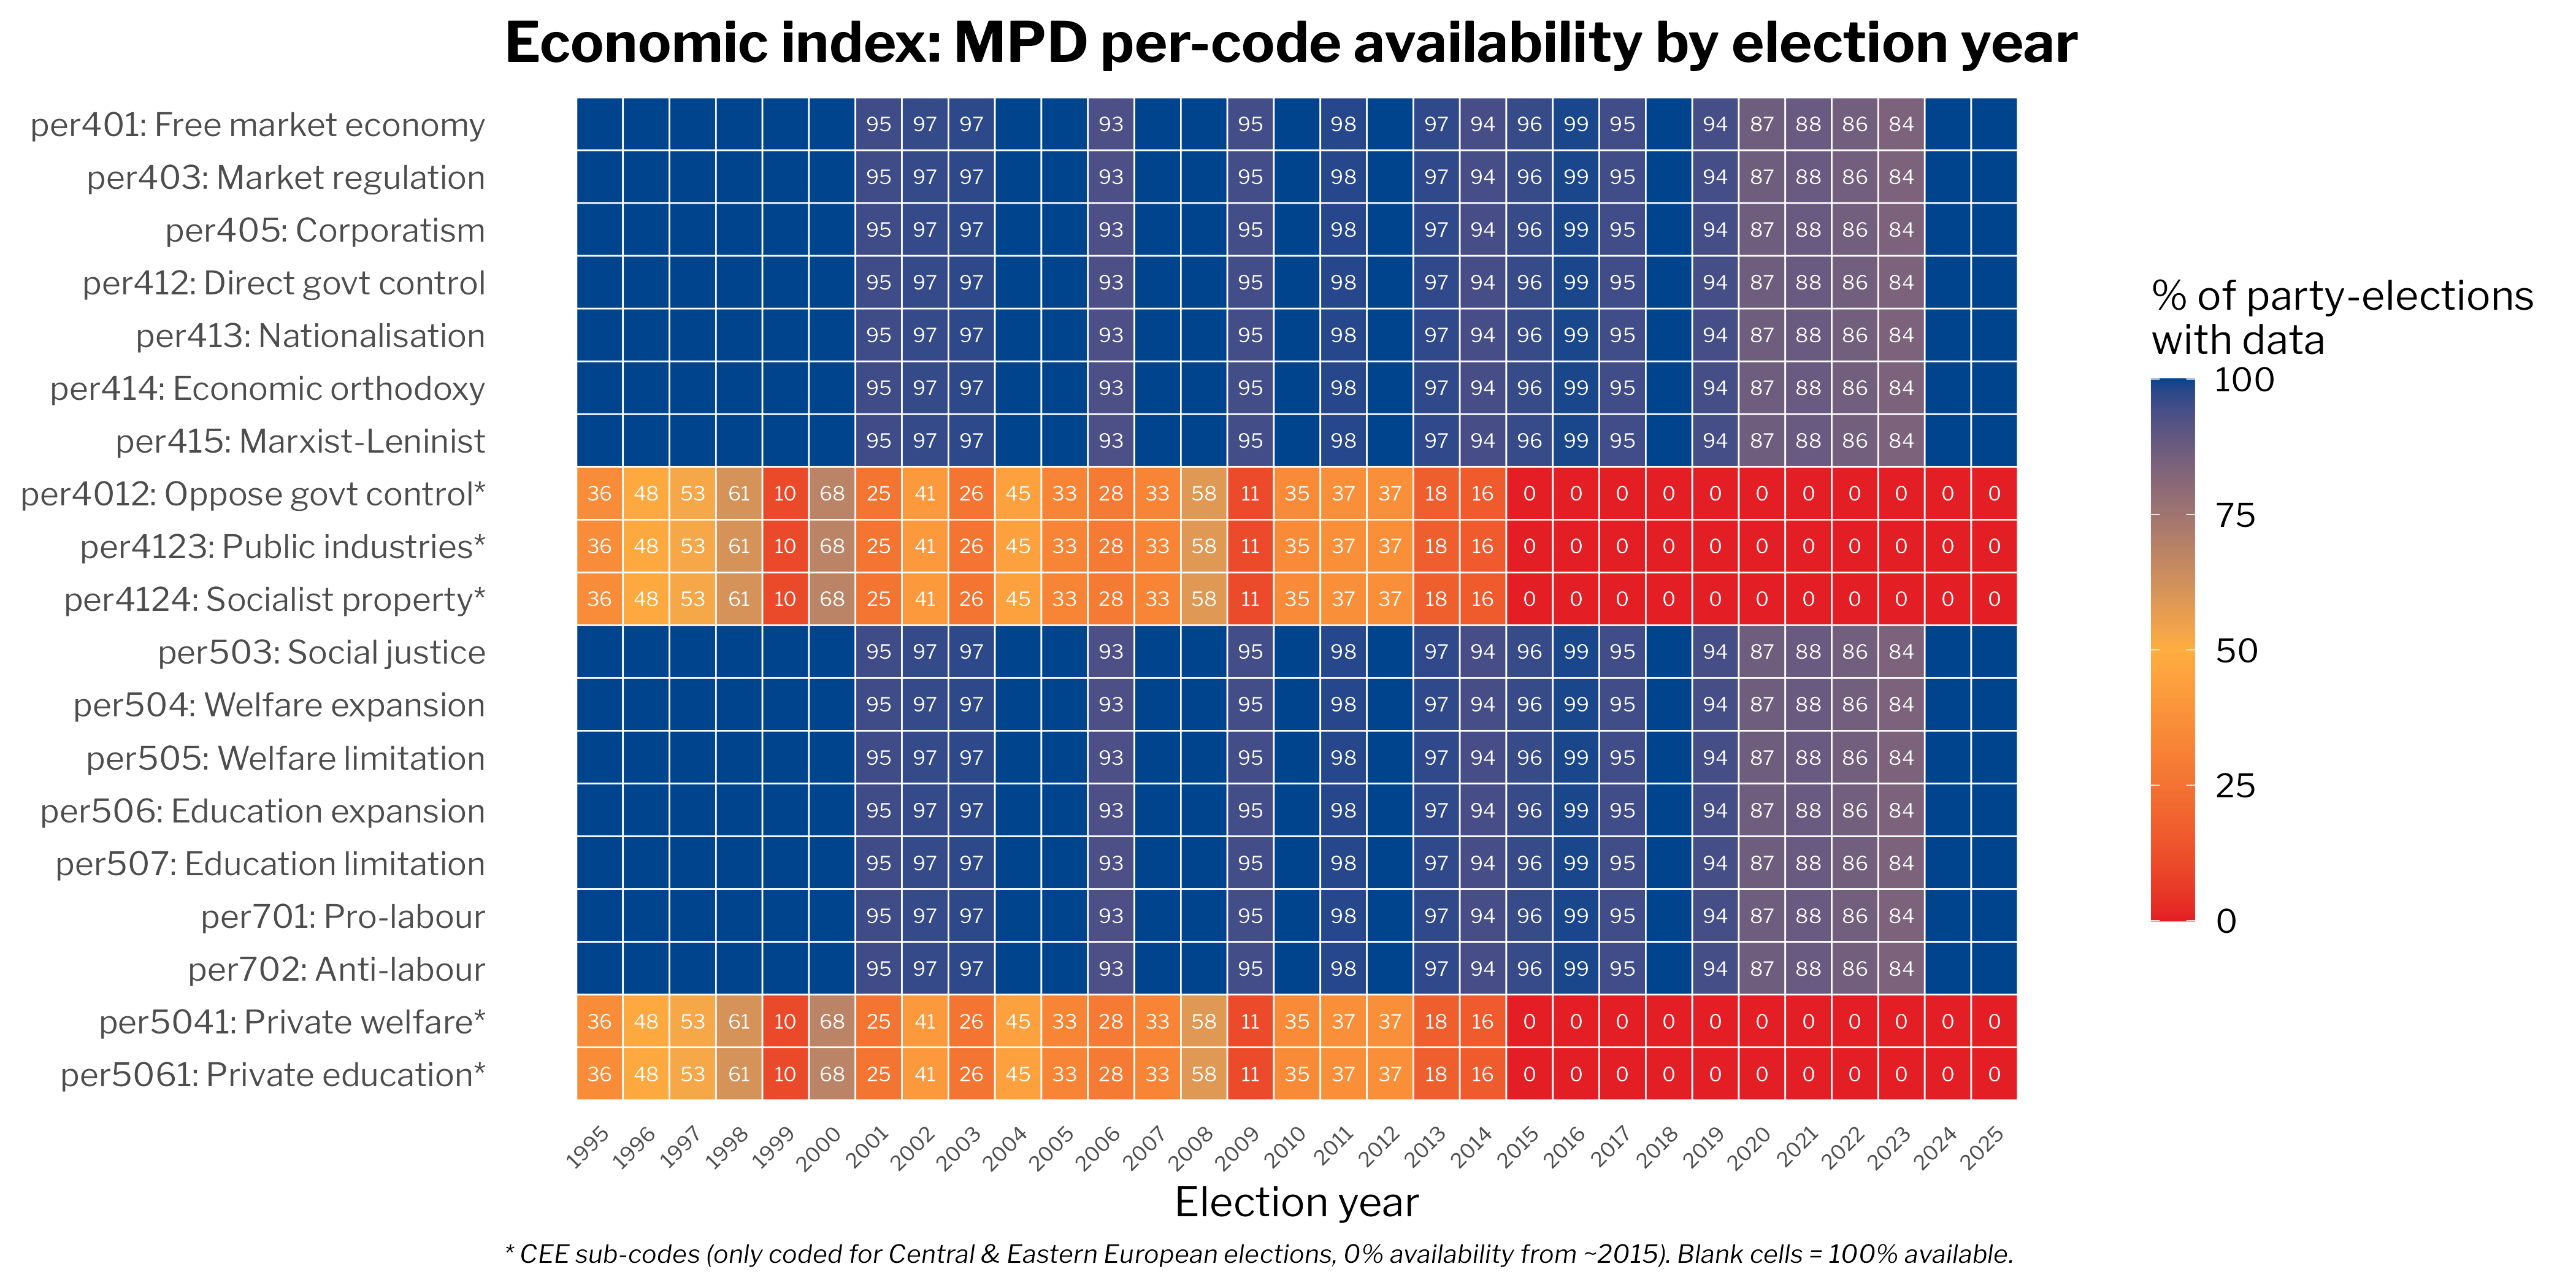
\includegraphics[width=1\textwidth]{../output/figures/mpd_coverage_economic.png}
%     \end{center}
% \end{figure}
%
% \end{frame} % ---------------------------------------------------------
%
%
% \begin{frame} % ---------------------------------------------------------
% \frametitle{Appendix: Cultural index per-code availability}\label{appendix:coverage_cult}
%
% \begin{figure}[H]
%     \begin{center}
%     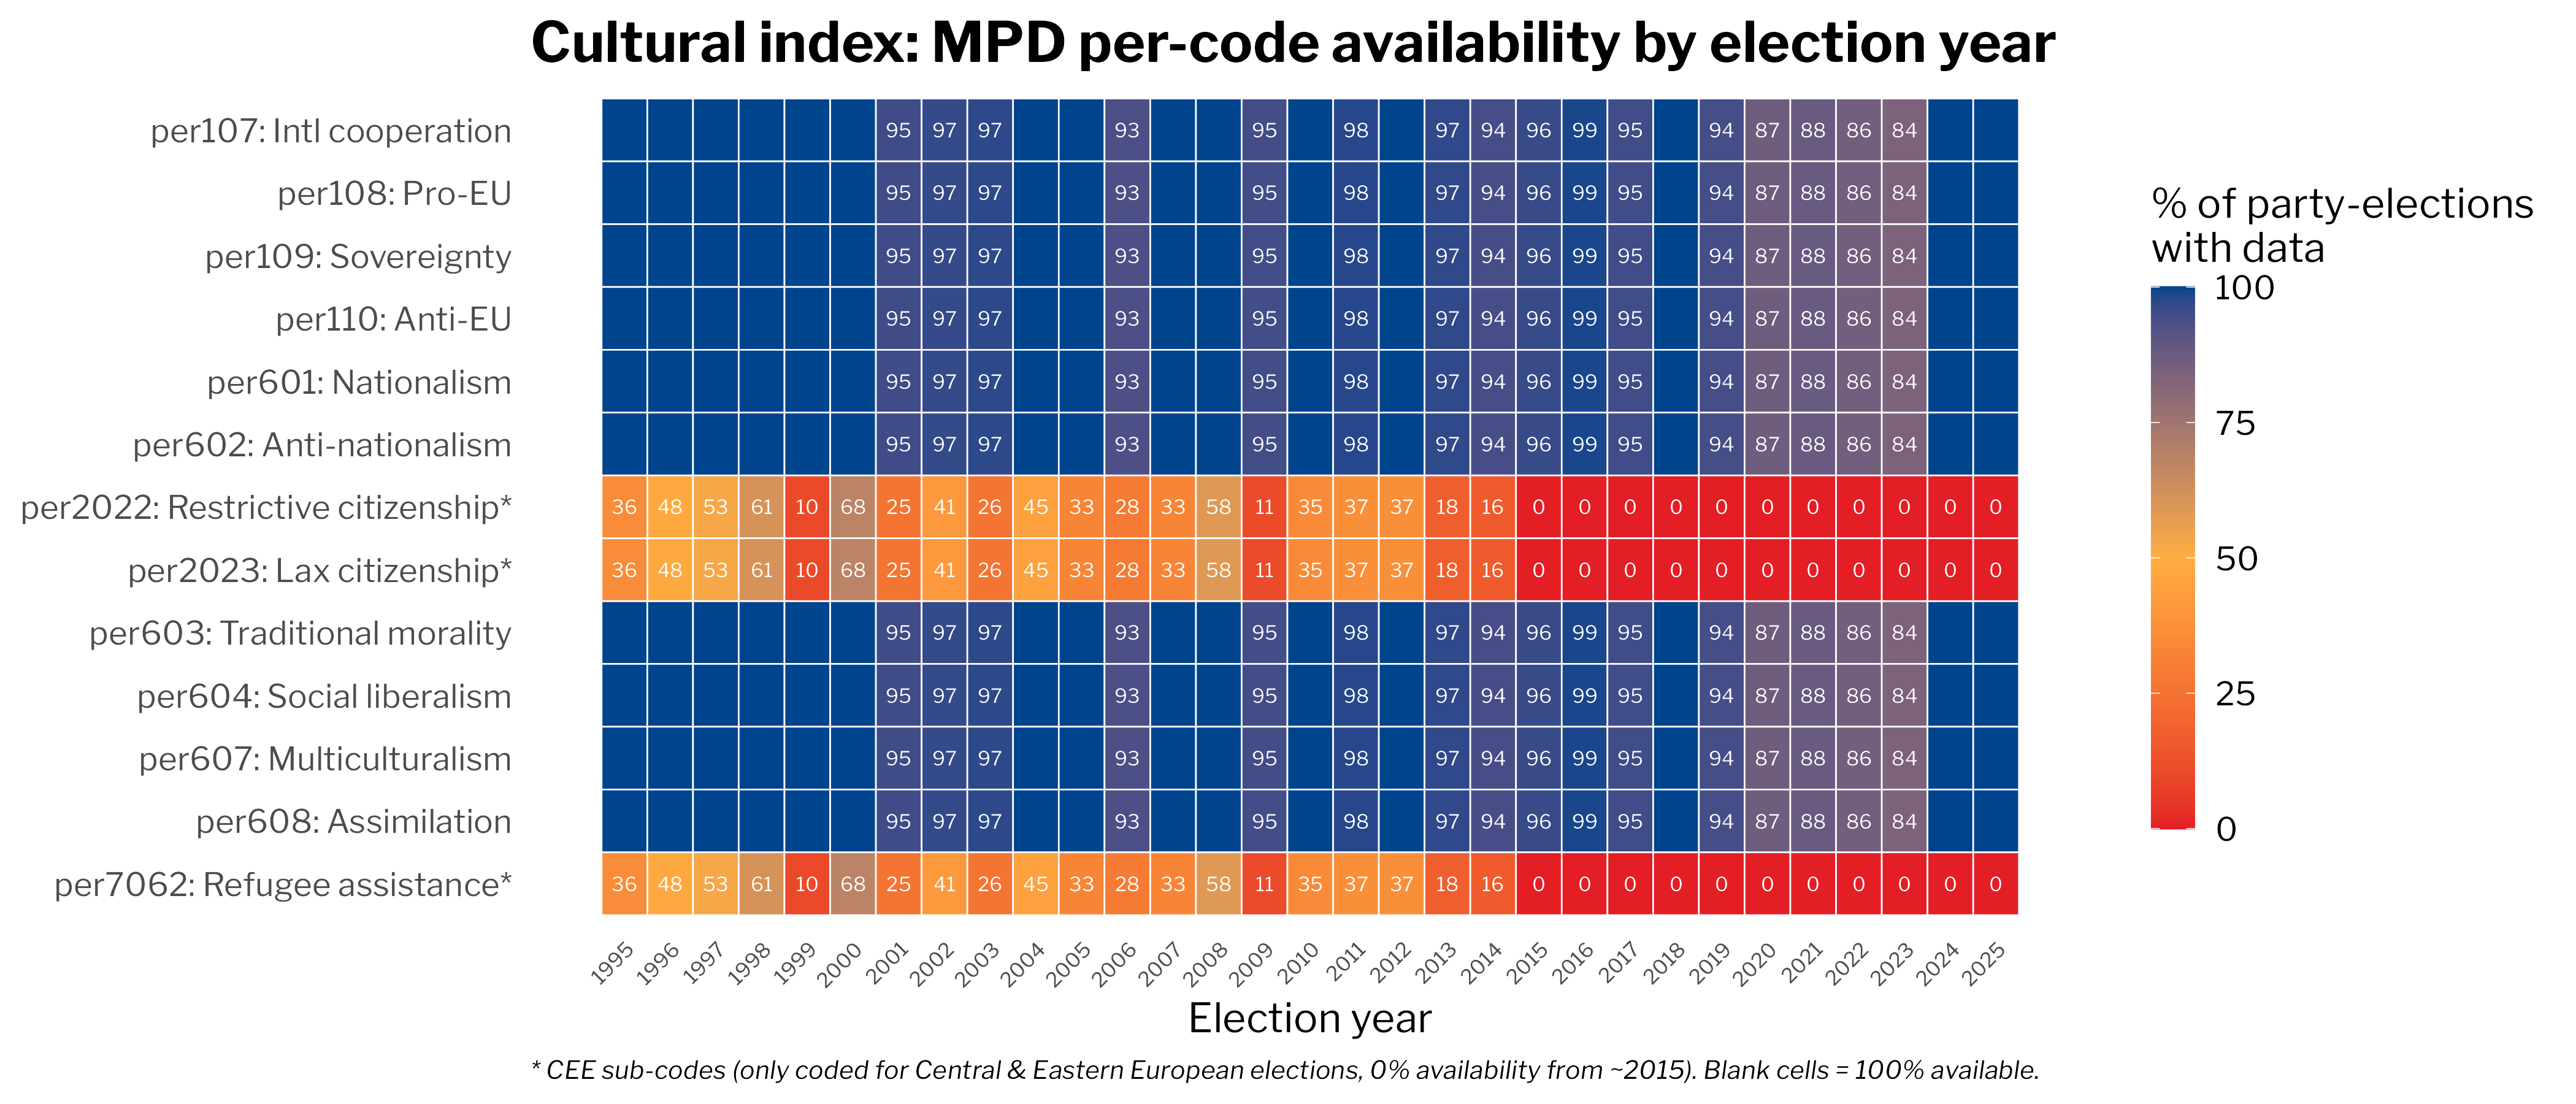
\includegraphics[width=1\textwidth]{../output/figures/mpd_coverage_cultural.png}
%     \end{center}
% \end{figure}
%
% \end{frame} % ---------------------------------------------------------

\end{document}
